% -*- latex -*-
%%%%%%%%%%%%%%%%%%%%%%%%%%%%%%%%%%%%%%%%%%%%%%%%%%%%%%%%%%%%%%%%
%%%%%%%%%%%%%%%%%%%%%%%%%%%%%%%%%%%%%%%%%%%%%%%%%%%%%%%%%%%%%%%%
%%%%
%%%% This text file is part of the source of 
%%%% `Parallel Programming in MPI and OpenMP'
%%%% by Victor Eijkhout, copyright 2012-9
%%%%
%%%% mpi-alltoall.tex : remarks about all-to-all
%%%%
%%%%%%%%%%%%%%%%%%%%%%%%%%%%%%%%%%%%%%%%%%%%%%%%%%%%%%%%%%%%%%%%
%%%%%%%%%%%%%%%%%%%%%%%%%%%%%%%%%%%%%%%%%%%%%%%%%%%%%%%%%%%%%%%%

\Level 0 {All-to-all}
\label{sec:alltoall}

The all-to-all operation can be seen as a collection of simultaneous
broadcasts or simultaneous gathers. The parameter specification is much
like an allgather, with a separate send and receive buffer, and no
root specified. As with the gather call, the receive count corresponds
to an individual receive, not the total amount.

Unlike the gather call, the send buffer now obeys the same principle:
with a send count of~1, the buffer has a length of the number of
processes.

\mpiRoutineRef{MPI_Alltoall}

\Level 1 {All-to-all as data transpose}
\label{sec:alltoall-transpose}

\begin{figure}[ht]
  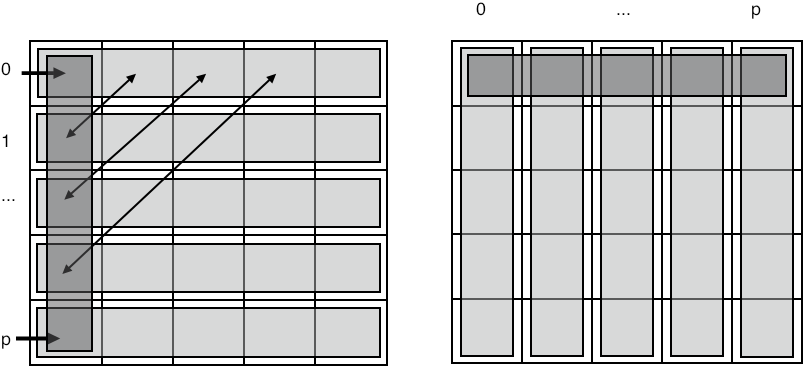
\includegraphics[scale=.4]{alltoall}
  \caption{All-to-all transposes data}
  \label{fig:alltoall}
\end{figure}

The all-to-all operation can be considered as a data transpose. For
instance, assume that each process knows how much data to send to
every other process. If you draw a connectivity matrix of size $P\times P$,
denoting who-sends-to-who, then the send information can be put in
rows:
\[ \forall_i\colon C[i,j]>0\quad\hbox{if process $i$ sends to process $j$}. \]
Conversely, the columns then denote the receive information:
\[ \forall_j\colon C[i,j]>0\quad\hbox{if process $j$ receives from process $i$}. \]

\begin{exercise}
  \label{ex:radixsort1}
  In the initial stage of \indextermsub{radix}{sorting}, each process
  considers how many elements to send to every other process.
  Use \indexmpishow{MPI_Alltoall} to derive from this how many
  elements they will receive from every other process.
\end{exercise}

On a larger scale, the typical application for the all-to-all
operation is in the \ac{FFT} algorithm, where it can take tens of
percents of the running time.

\Level 1 {All-to-all-v}

\begin{exercise}
  \label{ex:radixsort2}
  The actual data shuffle of a \indextermsub{radix}{sort} can be done
  with \indexmpishow{MPI_Alltoallv}. Finish the code of
  exercise~\ref{ex:radixsort1}.
\end{exercise}

\Level 0 {Reduce-scatter}
\label{sec:reducescatter}

There are several MPI collectives that are functionally equivalent to
a combination of others. You have already seen \indexmpishow{MPI_Allreduce} which
is equivalent to a reduction followed by a broadcast. Often such
combinations can be more efficient than using the individual calls;
see~\HPSCref{sec:collective}.

Here is another example: \indexmpishow{MPI_Reduce_scatter} is equivalent
to a reduction on an array of data (meaning a pointwise reduction on each
array location) followed by a scatter of this array to the individual 
processes.

\begin{figure}[ht]
  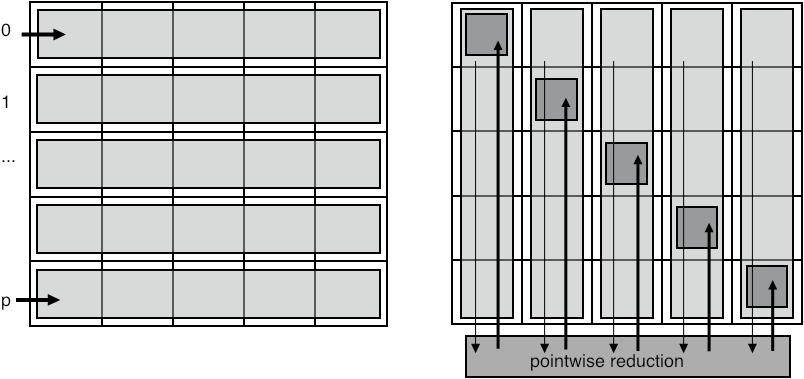
\includegraphics[scale=.4]{reducescatter}
  \caption{Reduce scatter}
  \label{fig:reducescatter}
\end{figure}

We can look at reduce-scatter as a limited form of the all-to-all data
transposition discussed above (section~\ref{sec:alltoall-transpose}).
Suppose that the matrix~$C$ contains only~$0/1$, indicating
whether or not a messages is send, rather than the actual amounts.
If a receiving process only needs to know how many messages to
receive, rather than where they come from, it is enough to know the
column sum, rather than the full column (see figure~\ref{fig:reducescatter}).

One important example of this command is the
\indextermsub{sparse}{matrix-vector product};
see~\HPSCref{sec:spmvp-performance} for background information.
Each process contains one or more matrix rows, so by looking at indices
the process can decide what other processes it needs data from.
The problem is for a process to find out what other processes 
it needs to send data to. 

Using \indexmpishow{MPI_Reduce_scatter} the process goes as follows:
\begin{itemize}
\item Each process creates an array of ones and zeros, describing who
  it needs data from.
\item The reduce part of the reduce-scatter yields an array of
  requester counts; after the scatter each process knows how many
  processes request data from it.
\item Next, the sender processes need to find out what elements are
  requested from it. For this, each process sends out arrays of
  indices.
\item The big trick is that each process now knows how many of these
  requests will be coming in, so it can post precisely that many
  \indexmpishow{MPI_Irecv} calls, with a source of \indexmpishow{MPI_ANY_SOURCE}.
\end{itemize}

The \indexmpishow{MPI_Reduce_scatter} command is equivalent to a reduction
on an array of data, followed by a scatter of that data to the individual processes.

To be precise, there is an array \n{recvcounts} where \n{recvcounts[i]} gives
the number of elements that ultimate wind up on process~\n{i}.
The result is equivalent to doing a reduction with a length equal to the sum
of the \n{recvcounts[i]} values, followed by a scatter where process~\n{i}
receives \n{recvcounts[i]} values. (Since the amount of data to be scattered
depends on the process, this is in fact equivalent to \indexmpishow{MPI_Scatterv}
rather than a regular scatter.)
%
\mpiRoutineRef{MPI_Reduce_scatter}
%
For instance, if all \n{recvcounts[i]} values are~1, the sendbuffer has one element
for each process, and the receive buffer has length~1.

\Level 1 {Examples}

An important application of this is establishing an irregular
communication pattern.  Assume that each process knows which
other processes it wants to communicate with; the problem is to
let the other processes know about this.
The solution is to use \indexmpishow{MPI_Reduce_scatter} to find out how many processes
want to communicate with you, and then wait for precisely that many messages
with a source value of \indexmpishow{MPI_ANY_SOURCE}.
\cverbatimsnippet[examples/mpi/c/reducescatter.c]{reducescatter}

Use of \indexmpishow{MPI_Reduce_scatter} to implement the two-dimensional
matrix-vector product.
Set up separate row and column communicators with
\indexmpishow{MPI_Comm_split}, use \indexmpishow{MPI_Reduce_scatter} to combine
local products.
%
\cverbatimsnippet[examples/mpi/c/mvp2d.c]{mvp2d}

\Level 0 {Barrier}
\label{sec:barrier}

A~barrier is a
routine that blocks all processes until they have all reached the barrier
call. Thus it achieves time synchronization of the processes.
%
\mpiRoutineRef{MPI_Barrier}
%
This call's simplicity is contrasted with its usefulness, which
is very limited. It is almost never necessary to synchronize processes
through a barrier: for most purposes it does not matter if processors
are out of sync. Conversely, collectives (except the new non-blocking
ones; section~\ref{sec:mpi3collect}) introduce a barrier of sorts themselves.

